\documentclass{article}
\usepackage[a4paper,margin=1in]{geometry}
\usepackage{amsmath}
\usepackage{amssymb}
\usepackage{graphicx}
\usepackage{tikz}
\usetikzlibrary{arrows.meta,automata,positioning}

\title{CSE411 Assignment \#2: Applying the Subset Construction Algorithm to \texttt{IF \(\mid\) ID \(\mid\) INT}}
\author{Sungho Kim (20241065)}
\date{\today}

\begin{document}
\maketitle

\section{NFA}
\begin{center}
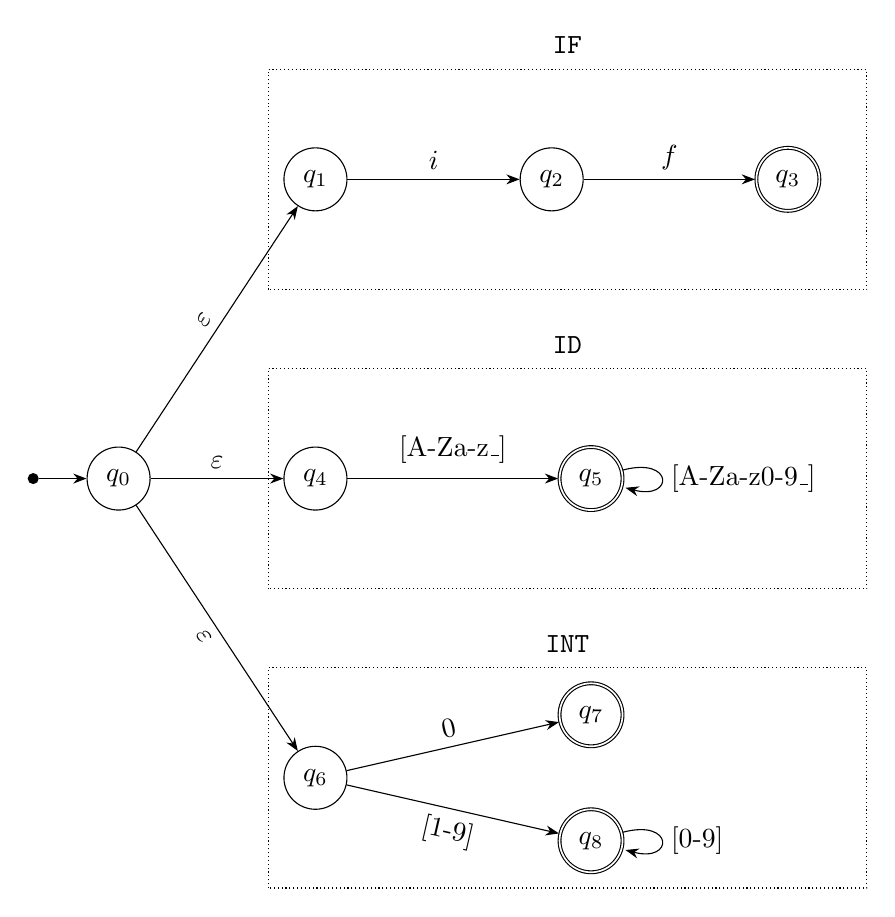
\begin{tikzpicture}[->, >=Stealth, every state/.style={minimum size=8mm}]
\node[state] (q0) at (0,0) {$q_0$};
\node[state] (q1) at (2.5,3.8) {$q_1$};
\node[state] (q2) at (5.5,3.8) {$q_2$};
\node[state, accepting] (q3) at (8.5,3.8) {$q_3$};
\node[state] (q4) at (2.5,0) {$q_4$};
\node[state, accepting] (q5) at (6,0) {$q_5$};
\node[state] (q6) at (2.5,-3.8) {$q_6$};
\node[state, accepting] (q7) at (6,-3) {$q_7$};
\node[state, accepting] (q8) at (6,-4.6) {$q_8$};
\node[circle, fill=black, inner sep=0pt, minimum size=4pt, left=6mm of q0] (start) {};
\draw (start) -- (q0);
\path (q0) edge node[above, sloped] {$\varepsilon$} (q1);
\path (q0) edge node[above] {$\varepsilon$} (q4);
\path (q0) edge node[below, sloped] {$\varepsilon$} (q6);
\path (q1) edge node[above] {$i$} (q2);
\path (q2) edge node[above] {$f$} (q3);
\path (q4) edge node[above=2pt] {[A-Za-z\_]} (q5);
\path (q5) edge[loop right] node[right] {[A-Za-z0-9\_]} (q5);
\path (q6) edge node[above, sloped] {$0$} (q7);
\path (q6) edge node[below, sloped] {[1-9]} (q8);
\path (q8) edge[loop right] node[right] {[0-9]} (q8);
\draw[densely dotted, -] (1.9,2.4) rectangle (9.5,5.2);
\node[above=2pt] at (5.7,5.2) {\texttt{IF}};
\draw[densely dotted, -] (1.9,-1.4) rectangle (9.5,1.4);
\node[above=2pt] at (5.7,1.4) {\texttt{ID}};
\draw[densely dotted, -] (1.9,-5.2) rectangle (9.5,-2.4);
\node[above=2pt] at (5.7,-2.4) {\texttt{INT}};
\end{tikzpicture}
\end{center}

\section{Step-by-Step Conversion to DFA}
\subsection{Identifying \texttt{D0, D, W}, and \texttt{F\_N}}
\begin{center}
\begin{tabular}{l|l}
\textbf{variable} & \textbf{value} \\
\hline
\(\mathtt{N0}\) & \(q_0\) \\
\(\mathtt{D0}\) & \(\varepsilon\mbox{-closure}(\{\mathtt{N0}\}) = \varepsilon\mbox{-closure}(\{q_0\}) = \{q_0, q_1, q_4, q_6\}\) \\
\texttt{D} & \(\{\mathtt{D0}\} = \bigl\{\{q_0, q_1, q_4, q_6\}\bigr\}\) \\
\texttt{W} & \(\{\mathtt{D0}\} = \bigl\{\{q_0, q_1, q_4, q_6\}\bigr\}\) \\
\texttt{F\_N} & \(\{q_3, q_5, q_7, q_8\}\) \\
\end{tabular}
\end{center}

\subsection{Intermediate Automata}
\par\medskip\noindent
\begin{minipage}[c]{0.59\textwidth}
\scriptsize
\setlength{\tabcolsep}{2pt}
\renewcommand{\arraystretch}{1.45}
\begin{tabular}{@{}p{0.13\linewidth}|p{0.39\linewidth}|p{\dimexpr0.48\linewidth-4\tabcolsep-2\arrayrulewidth\relax}@{}}
\textbf{line} & \textbf{operation} & \textbf{value} \\
\hline
1 & \(\mathtt{D0} := \varepsilon\mbox{-closure}(\{\mathtt{N0}\})\) & \(\mathtt{D0}=Q_0=\{q_0,q_1,q_4,q_6\}\) \\
2 & \(\mathtt{D} := \{\mathtt{D0}\}\) & \(\mathtt{D}=\{Q_0\}\) \\
\end{tabular}
\end{minipage}\hfill%
\begin{minipage}[c]{0.39\textwidth}
\centering
\resizebox{\linewidth}{!}{%
\begin{tikzpicture}[->, >=Stealth, every state/.style={minimum size=8mm}]
\path[use as bounding box] (-0.9,-5) rectangle (12.2,3.2);
\node[state] (Q0) at (0,0) {$Q_0$};
\node[circle, fill=black, inner sep=0pt, minimum size=4pt, left=6mm of Q0] (start) {};
\draw (start) -- (Q0);
\end{tikzpicture}
}
\end{minipage}
\par\medskip
\par\medskip\noindent
\begin{minipage}[c]{0.59\textwidth}
\scriptsize
\setlength{\tabcolsep}{2pt}
\renewcommand{\arraystretch}{1.45}
\begin{tabular}{@{}p{0.13\linewidth}|p{0.39\linewidth}|p{\dimexpr0.48\linewidth-4\tabcolsep-2\arrayrulewidth\relax}@{}}
\textbf{line} & \textbf{operation} & \textbf{value} \\
\hline
3 & \(\mathtt{W} := \{\mathtt{D0}\}\) & \(\mathtt{W}=\{Q_0\}\) \\
4 & \(\textbf{while }\mathtt{W}\ne\emptyset\) & \(\mathtt{W}=\{Q_0\}\ne\emptyset\) \\
5 & \(\textbf{remove }\mathtt{Q}\textbf{ from }\mathtt{W}\) & \(\mathtt{Q}=Q_0,\quad \mathtt{W}=\{\}\) \\
6 & \(\textbf{for }\alpha\in\Sigma\) & \(\alpha=i\) \\
7 & \(\mathtt{T} := \emptyset\) & \(\mathtt{T}=\emptyset\) \\
8 & \(\textbf{for }\mathtt{S}\in\mathtt{Q}\) & \(\mathtt{S}=q_0\) \\
9 & \(\mathtt{T} := \mathtt{T}\cup\delta_N(\mathtt{S},\alpha)\) & \(\emptyset\to\emptyset\) \\
8 & \(\textbf{for }\mathtt{S}\in\mathtt{Q}\) & \(\mathtt{S}=q_1\) \\
9 & \(\mathtt{T} := \mathtt{T}\cup\delta_N(\mathtt{S},\alpha)\) & \(\emptyset\to\{q_2\}\) \\
8 & \(\textbf{for }\mathtt{S}\in\mathtt{Q}\) & \(\mathtt{S}=q_4\) \\
9 & \(\mathtt{T} := \mathtt{T}\cup\delta_N(\mathtt{S},\alpha)\) & \(\{q_2\}\to\{q_2,q_5\}\) \\
8 & \(\textbf{for }\mathtt{S}\in\mathtt{Q}\) & \(\mathtt{S}=q_6\) \\
9 & \(\mathtt{T} := \mathtt{T}\cup\delta_N(\mathtt{S},\alpha)\) & \(\{q_2,q_5\}\to\{q_2,q_5\}\) \\
10 & \(\mathtt{T}' := \varepsilon\mbox{-closure}(\mathtt{T})\) & \(\mathtt{T}'=\{q_2,q_5\}=Q_1\) \\
11 & \(\mathtt{D}' := \mathtt{D}\cup\{\mathtt{T}'\}\) & \(\mathtt{D}'=\{Q_0,Q_1\}\) \\
\end{tabular}
\end{minipage}\hfill%
\begin{minipage}[c]{0.39\textwidth}
\centering
\resizebox{\linewidth}{!}{%
\begin{tikzpicture}[->, >=Stealth, every state/.style={minimum size=8mm}]
\path[use as bounding box] (-0.9,-5) rectangle (12.2,3.2);
\node[state] (Q0) at (0,0) {$Q_0$};
\node[state] (Q1) at (30:5) {$Q_1$};
\node[circle, fill=black, inner sep=0pt, minimum size=4pt, left=6mm of Q0] (start) {};
\draw (start) -- (Q0);
\end{tikzpicture}
}
\end{minipage}
\par\medskip
\par\medskip\noindent
\begin{minipage}[c]{0.59\textwidth}
\scriptsize
\setlength{\tabcolsep}{2pt}
\renewcommand{\arraystretch}{1.45}
\begin{tabular}{@{}p{0.13\linewidth}|p{0.39\linewidth}|p{\dimexpr0.48\linewidth-4\tabcolsep-2\arrayrulewidth\relax}@{}}
\textbf{line} & \textbf{operation} & \textbf{value} \\
\hline
12 & \(\delta_D(\mathtt{Q},\alpha) := \mathtt{T}'\) & \(\delta_D(Q_0,\alpha)=Q_1\) \\
\end{tabular}
\end{minipage}\hfill%
\begin{minipage}[c]{0.39\textwidth}
\centering
\resizebox{\linewidth}{!}{%
\begin{tikzpicture}[->, >=Stealth, every state/.style={minimum size=8mm}]
\path[use as bounding box] (-0.9,-5) rectangle (12.2,3.2);
\node[state] (Q0) at (0,0) {$Q_0$};
\node[state] (Q1) at (30:5) {$Q_1$};
\node[circle, fill=black, inner sep=0pt, minimum size=4pt, left=6mm of Q0] (start) {};
\draw (start) -- (Q0);
\path (Q0) edge node[midway, align=center, above, sloped] {$i$} (Q1);
\end{tikzpicture}
}
\end{minipage}
\par\medskip
\par\medskip\noindent
\begin{minipage}[c]{0.59\textwidth}
\scriptsize
\setlength{\tabcolsep}{2pt}
\renewcommand{\arraystretch}{1.45}
\begin{tabular}{@{}p{0.13\linewidth}|p{0.39\linewidth}|p{\dimexpr0.48\linewidth-4\tabcolsep-2\arrayrulewidth\relax}@{}}
\textbf{line} & \textbf{operation} & \textbf{value} \\
\hline
13 & \(\textbf{if }\mathtt{T}'\notin\mathtt{D}\) & \(Q_1\notin\mathtt{D}\) \\
14 & \(\mathtt{W} := \mathtt{W}\cup\{\mathtt{T}'\}\) & \(\mathtt{W}=\{Q_1\}\) \\
15 & \(\mathtt{D} := \mathtt{D}'\) & \(\mathtt{D}=\{Q_0,Q_1\}\) \\
6 & \(\textbf{for }\alpha\in\Sigma\) & \(\alpha\in\) [A-Za-z\_] $-$ $\{i\}$ \\
7 & \(\mathtt{T} := \emptyset\) & \(\mathtt{T}=\emptyset\) \\
8 & \(\textbf{for }\mathtt{S}\in\mathtt{Q}\) & \(\mathtt{S}=q_0\) \\
9 & \(\mathtt{T} := \mathtt{T}\cup\delta_N(\mathtt{S},\alpha)\) & \(\emptyset\to\emptyset\) \\
8 & \(\textbf{for }\mathtt{S}\in\mathtt{Q}\) & \(\mathtt{S}=q_1\) \\
9 & \(\mathtt{T} := \mathtt{T}\cup\delta_N(\mathtt{S},\alpha)\) & \(\emptyset\to\emptyset\) \\
8 & \(\textbf{for }\mathtt{S}\in\mathtt{Q}\) & \(\mathtt{S}=q_4\) \\
9 & \(\mathtt{T} := \mathtt{T}\cup\delta_N(\mathtt{S},\alpha)\) & \(\emptyset\to\{q_5\}\) \\
8 & \(\textbf{for }\mathtt{S}\in\mathtt{Q}\) & \(\mathtt{S}=q_6\) \\
9 & \(\mathtt{T} := \mathtt{T}\cup\delta_N(\mathtt{S},\alpha)\) & \(\{q_5\}\to\{q_5\}\) \\
10 & \(\mathtt{T}' := \varepsilon\mbox{-closure}(\mathtt{T})\) & \(\mathtt{T}'=\{q_5\}=Q_3\) \\
11 & \(\mathtt{D}' := \mathtt{D}\cup\{\mathtt{T}'\}\) & \(\mathtt{D}'=\{Q_0,Q_1,Q_3\}\) \\
\end{tabular}
\end{minipage}\hfill%
\begin{minipage}[c]{0.39\textwidth}
\centering
\resizebox{\linewidth}{!}{%
\begin{tikzpicture}[->, >=Stealth, every state/.style={minimum size=8mm}]
\path[use as bounding box] (-0.9,-5) rectangle (12.2,3.2);
\node[state] (Q0) at (0,0) {$Q_0$};
\node[state] (Q1) at (30:5) {$Q_1$};
\node[state] (Q3) at (9,0) {$Q_3$};
\node[circle, fill=black, inner sep=0pt, minimum size=4pt, left=6mm of Q0] (start) {};
\draw (start) -- (Q0);
\path (Q0) edge node[midway, align=center, above, sloped] {$i$} (Q1);
\end{tikzpicture}
}
\end{minipage}
\par\medskip
\par\medskip\noindent
\begin{minipage}[c]{0.59\textwidth}
\scriptsize
\setlength{\tabcolsep}{2pt}
\renewcommand{\arraystretch}{1.45}
\begin{tabular}{@{}p{0.13\linewidth}|p{0.39\linewidth}|p{\dimexpr0.48\linewidth-4\tabcolsep-2\arrayrulewidth\relax}@{}}
\textbf{line} & \textbf{operation} & \textbf{value} \\
\hline
12 & \(\delta_D(\mathtt{Q},\alpha) := \mathtt{T}'\) & \(\delta_D(Q_0,\alpha)=Q_3\) \\
\end{tabular}
\end{minipage}\hfill%
\begin{minipage}[c]{0.39\textwidth}
\centering
\resizebox{\linewidth}{!}{%
\begin{tikzpicture}[->, >=Stealth, every state/.style={minimum size=8mm}]
\path[use as bounding box] (-0.9,-5) rectangle (12.2,3.2);
\node[state] (Q0) at (0,0) {$Q_0$};
\node[state] (Q1) at (30:5) {$Q_1$};
\node[state] (Q3) at (9,0) {$Q_3$};
\node[circle, fill=black, inner sep=0pt, minimum size=4pt, left=6mm of Q0] (start) {};
\draw (start) -- (Q0);
\path (Q0) edge node[midway, align=center, above, sloped] {$i$} (Q1);
\path (Q0) edge node[midway, align=center, above=2pt] {[A-Za-z\_] $-$ $\{i\}$} (Q3);
\end{tikzpicture}
}
\end{minipage}
\par\medskip
\par\medskip\noindent
\begin{minipage}[c]{0.59\textwidth}
\scriptsize
\setlength{\tabcolsep}{2pt}
\renewcommand{\arraystretch}{1.45}
\begin{tabular}{@{}p{0.13\linewidth}|p{0.39\linewidth}|p{\dimexpr0.48\linewidth-4\tabcolsep-2\arrayrulewidth\relax}@{}}
\textbf{line} & \textbf{operation} & \textbf{value} \\
\hline
13 & \(\textbf{if }\mathtt{T}'\notin\mathtt{D}\) & \(Q_3\notin\mathtt{D}\) \\
14 & \(\mathtt{W} := \mathtt{W}\cup\{\mathtt{T}'\}\) & \(\mathtt{W}=\{Q_1,Q_3\}\) \\
15 & \(\mathtt{D} := \mathtt{D}'\) & \(\mathtt{D}=\{Q_0,Q_1,Q_3\}\) \\
6 & \(\textbf{for }\alpha\in\Sigma\) & \(\alpha=0\) \\
7 & \(\mathtt{T} := \emptyset\) & \(\mathtt{T}=\emptyset\) \\
8 & \(\textbf{for }\mathtt{S}\in\mathtt{Q}\) & \(\mathtt{S}=q_0\) \\
9 & \(\mathtt{T} := \mathtt{T}\cup\delta_N(\mathtt{S},\alpha)\) & \(\emptyset\to\emptyset\) \\
8 & \(\textbf{for }\mathtt{S}\in\mathtt{Q}\) & \(\mathtt{S}=q_1\) \\
9 & \(\mathtt{T} := \mathtt{T}\cup\delta_N(\mathtt{S},\alpha)\) & \(\emptyset\to\emptyset\) \\
8 & \(\textbf{for }\mathtt{S}\in\mathtt{Q}\) & \(\mathtt{S}=q_4\) \\
9 & \(\mathtt{T} := \mathtt{T}\cup\delta_N(\mathtt{S},\alpha)\) & \(\emptyset\to\emptyset\) \\
8 & \(\textbf{for }\mathtt{S}\in\mathtt{Q}\) & \(\mathtt{S}=q_6\) \\
9 & \(\mathtt{T} := \mathtt{T}\cup\delta_N(\mathtt{S},\alpha)\) & \(\emptyset\to\{q_7\}\) \\
10 & \(\mathtt{T}' := \varepsilon\mbox{-closure}(\mathtt{T})\) & \(\mathtt{T}'=\{q_7\}=Q_4\) \\
11 & \(\mathtt{D}' := \mathtt{D}\cup\{\mathtt{T}'\}\) & \(\mathtt{D}'=\{Q_0,Q_1,Q_3,Q_4\}\) \\
\end{tabular}
\end{minipage}\hfill%
\begin{minipage}[c]{0.39\textwidth}
\centering
\resizebox{\linewidth}{!}{%
\begin{tikzpicture}[->, >=Stealth, every state/.style={minimum size=8mm}]
\path[use as bounding box] (-0.9,-5) rectangle (12.2,3.2);
\node[state] (Q0) at (0,0) {$Q_0$};
\node[state] (Q1) at (30:5) {$Q_1$};
\node[state] (Q3) at (9,0) {$Q_3$};
\node[state] (Q4) at (-30:5) {$Q_4$};
\node[circle, fill=black, inner sep=0pt, minimum size=4pt, left=6mm of Q0] (start) {};
\draw (start) -- (Q0);
\path (Q0) edge node[midway, align=center, above, sloped] {$i$} (Q1);
\path (Q0) edge node[midway, align=center, above=2pt] {[A-Za-z\_] $-$ $\{i\}$} (Q3);
\end{tikzpicture}
}
\end{minipage}
\par\medskip
\par\medskip\noindent
\begin{minipage}[c]{0.59\textwidth}
\scriptsize
\setlength{\tabcolsep}{2pt}
\renewcommand{\arraystretch}{1.45}
\begin{tabular}{@{}p{0.13\linewidth}|p{0.39\linewidth}|p{\dimexpr0.48\linewidth-4\tabcolsep-2\arrayrulewidth\relax}@{}}
\textbf{line} & \textbf{operation} & \textbf{value} \\
\hline
12 & \(\delta_D(\mathtt{Q},\alpha) := \mathtt{T}'\) & \(\delta_D(Q_0,\alpha)=Q_4\) \\
\end{tabular}
\end{minipage}\hfill%
\begin{minipage}[c]{0.39\textwidth}
\centering
\resizebox{\linewidth}{!}{%
\begin{tikzpicture}[->, >=Stealth, every state/.style={minimum size=8mm}]
\path[use as bounding box] (-0.9,-5) rectangle (12.2,3.2);
\node[state] (Q0) at (0,0) {$Q_0$};
\node[state] (Q1) at (30:5) {$Q_1$};
\node[state] (Q3) at (9,0) {$Q_3$};
\node[state] (Q4) at (-30:5) {$Q_4$};
\node[circle, fill=black, inner sep=0pt, minimum size=4pt, left=6mm of Q0] (start) {};
\draw (start) -- (Q0);
\path (Q0) edge node[midway, align=center, above, sloped] {$i$} (Q1);
\path (Q0) edge node[midway, align=center, above=2pt] {[A-Za-z\_] $-$ $\{i\}$} (Q3);
\path (Q0) edge node[midway, align=center, below, sloped] {$0$} (Q4);
\end{tikzpicture}
}
\end{minipage}
\par\medskip
\par\medskip\noindent
\begin{minipage}[c]{0.59\textwidth}
\scriptsize
\setlength{\tabcolsep}{2pt}
\renewcommand{\arraystretch}{1.45}
\begin{tabular}{@{}p{0.13\linewidth}|p{0.39\linewidth}|p{\dimexpr0.48\linewidth-4\tabcolsep-2\arrayrulewidth\relax}@{}}
\textbf{line} & \textbf{operation} & \textbf{value} \\
\hline
13 & \(\textbf{if }\mathtt{T}'\notin\mathtt{D}\) & \(Q_4\notin\mathtt{D}\) \\
14 & \(\mathtt{W} := \mathtt{W}\cup\{\mathtt{T}'\}\) & \(\mathtt{W}=\{Q_1,Q_3,Q_4\}\) \\
15 & \(\mathtt{D} := \mathtt{D}'\) & \(\mathtt{D}=\{Q_0,Q_1,Q_3,Q_4\}\) \\
6 & \(\textbf{for }\alpha\in\Sigma\) & \(\alpha\in\) [1-9] \\
7 & \(\mathtt{T} := \emptyset\) & \(\mathtt{T}=\emptyset\) \\
8 & \(\textbf{for }\mathtt{S}\in\mathtt{Q}\) & \(\mathtt{S}=q_0\) \\
9 & \(\mathtt{T} := \mathtt{T}\cup\delta_N(\mathtt{S},\alpha)\) & \(\emptyset\to\emptyset\) \\
8 & \(\textbf{for }\mathtt{S}\in\mathtt{Q}\) & \(\mathtt{S}=q_1\) \\
9 & \(\mathtt{T} := \mathtt{T}\cup\delta_N(\mathtt{S},\alpha)\) & \(\emptyset\to\emptyset\) \\
8 & \(\textbf{for }\mathtt{S}\in\mathtt{Q}\) & \(\mathtt{S}=q_4\) \\
9 & \(\mathtt{T} := \mathtt{T}\cup\delta_N(\mathtt{S},\alpha)\) & \(\emptyset\to\emptyset\) \\
8 & \(\textbf{for }\mathtt{S}\in\mathtt{Q}\) & \(\mathtt{S}=q_6\) \\
9 & \(\mathtt{T} := \mathtt{T}\cup\delta_N(\mathtt{S},\alpha)\) & \(\emptyset\to\{q_8\}\) \\
10 & \(\mathtt{T}' := \varepsilon\mbox{-closure}(\mathtt{T})\) & \(\mathtt{T}'=\{q_8\}=Q_5\) \\
11 & \(\mathtt{D}' := \mathtt{D}\cup\{\mathtt{T}'\}\) & \(\mathtt{D}'=\{Q_0,Q_1,Q_3,Q_4,Q_5\}\) \\
\end{tabular}
\end{minipage}\hfill%
\begin{minipage}[c]{0.39\textwidth}
\centering
\resizebox{\linewidth}{!}{%
\begin{tikzpicture}[->, >=Stealth, every state/.style={minimum size=8mm}]
\path[use as bounding box] (-0.9,-5) rectangle (12.2,3.2);
\node[state] (Q0) at (0,0) {$Q_0$};
\node[state] (Q1) at (30:5) {$Q_1$};
\node[state] (Q3) at (9,0) {$Q_3$};
\node[state] (Q4) at (-30:5) {$Q_4$};
\node[state] (Q5) at (-60:5) {$Q_5$};
\node[circle, fill=black, inner sep=0pt, minimum size=4pt, left=6mm of Q0] (start) {};
\draw (start) -- (Q0);
\path (Q0) edge node[midway, align=center, above, sloped] {$i$} (Q1);
\path (Q0) edge node[midway, align=center, above=2pt] {[A-Za-z\_] $-$ $\{i\}$} (Q3);
\path (Q0) edge node[midway, align=center, below, sloped] {$0$} (Q4);
\end{tikzpicture}
}
\end{minipage}
\par\medskip
\par\medskip\noindent
\begin{minipage}[c]{0.59\textwidth}
\scriptsize
\setlength{\tabcolsep}{2pt}
\renewcommand{\arraystretch}{1.45}
\begin{tabular}{@{}p{0.13\linewidth}|p{0.39\linewidth}|p{\dimexpr0.48\linewidth-4\tabcolsep-2\arrayrulewidth\relax}@{}}
\textbf{line} & \textbf{operation} & \textbf{value} \\
\hline
12 & \(\delta_D(\mathtt{Q},\alpha) := \mathtt{T}'\) & \(\delta_D(Q_0,\alpha)=Q_5\) \\
\end{tabular}
\end{minipage}\hfill%
\begin{minipage}[c]{0.39\textwidth}
\centering
\resizebox{\linewidth}{!}{%
\begin{tikzpicture}[->, >=Stealth, every state/.style={minimum size=8mm}]
\path[use as bounding box] (-0.9,-5) rectangle (12.2,3.2);
\node[state] (Q0) at (0,0) {$Q_0$};
\node[state] (Q1) at (30:5) {$Q_1$};
\node[state] (Q3) at (9,0) {$Q_3$};
\node[state] (Q4) at (-30:5) {$Q_4$};
\node[state] (Q5) at (-60:5) {$Q_5$};
\node[circle, fill=black, inner sep=0pt, minimum size=4pt, left=6mm of Q0] (start) {};
\draw (start) -- (Q0);
\path (Q0) edge node[midway, align=center, above, sloped] {$i$} (Q1);
\path (Q0) edge node[midway, align=center, above=2pt] {[A-Za-z\_] $-$ $\{i\}$} (Q3);
\path (Q0) edge node[midway, align=center, below, sloped] {$0$} (Q4);
\path (Q0) edge node[midway, align=center, below, sloped] {[1-9]} (Q5);
\end{tikzpicture}
}
\end{minipage}
\par\medskip
\par\medskip\noindent
\begin{minipage}[c]{0.59\textwidth}
\scriptsize
\setlength{\tabcolsep}{2pt}
\renewcommand{\arraystretch}{1.45}
\begin{tabular}{@{}p{0.13\linewidth}|p{0.39\linewidth}|p{\dimexpr0.48\linewidth-4\tabcolsep-2\arrayrulewidth\relax}@{}}
\textbf{line} & \textbf{operation} & \textbf{value} \\
\hline
13 & \(\textbf{if }\mathtt{T}'\notin\mathtt{D}\) & \(Q_5\notin\mathtt{D}\) \\
14 & \(\mathtt{W} := \mathtt{W}\cup\{\mathtt{T}'\}\) & \(\mathtt{W}=\{Q_1,Q_3,Q_4,Q_5\}\) \\
15 & \(\mathtt{D} := \mathtt{D}'\) & \(\mathtt{D}=\{Q_0,Q_1,Q_3,Q_4,Q_5\}\) \\
4 & \(\textbf{while }\mathtt{W}\ne\emptyset\) & \(\mathtt{W}=\{Q_1,Q_3,Q_4,Q_5\}\ne\emptyset\) \\
5 & \(\textbf{remove }\mathtt{Q}\textbf{ from }\mathtt{W}\) & \(\mathtt{Q}=Q_1,\quad \mathtt{W}=\{Q_3,Q_4,Q_5\}\) \\
6 & \(\textbf{for }\alpha\in\Sigma\) & \(\alpha=f\) \\
7 & \(\mathtt{T} := \emptyset\) & \(\mathtt{T}=\emptyset\) \\
8 & \(\textbf{for }\mathtt{S}\in\mathtt{Q}\) & \(\mathtt{S}=q_2\) \\
9 & \(\mathtt{T} := \mathtt{T}\cup\delta_N(\mathtt{S},\alpha)\) & \(\emptyset\to\{q_3\}\) \\
8 & \(\textbf{for }\mathtt{S}\in\mathtt{Q}\) & \(\mathtt{S}=q_5\) \\
9 & \(\mathtt{T} := \mathtt{T}\cup\delta_N(\mathtt{S},\alpha)\) & \(\{q_3\}\to\{q_3,q_5\}\) \\
10 & \(\mathtt{T}' := \varepsilon\mbox{-closure}(\mathtt{T})\) & \(\mathtt{T}'=\{q_3,q_5\}=Q_2\) \\
11 & \(\mathtt{D}' := \mathtt{D}\cup\{\mathtt{T}'\}\) & \(\mathtt{D}'=\{Q_0,Q_1,Q_2,Q_3,Q_4,Q_5\}\) \\
\end{tabular}
\end{minipage}\hfill%
\begin{minipage}[c]{0.39\textwidth}
\centering
\resizebox{\linewidth}{!}{%
\begin{tikzpicture}[->, >=Stealth, every state/.style={minimum size=8mm}]
\path[use as bounding box] (-0.9,-5) rectangle (12.2,3.2);
\node[state] (Q0) at (0,0) {$Q_0$};
\node[state] (Q1) at (30:5) {$Q_1$};
\node[state] (Q2) at (9,2.5) {$Q_2$};
\node[state] (Q3) at (9,0) {$Q_3$};
\node[state] (Q4) at (-30:5) {$Q_4$};
\node[state] (Q5) at (-60:5) {$Q_5$};
\node[circle, fill=black, inner sep=0pt, minimum size=4pt, left=6mm of Q0] (start) {};
\draw (start) -- (Q0);
\path (Q0) edge node[midway, align=center, above, sloped] {$i$} (Q1);
\path (Q0) edge node[midway, align=center, above=2pt] {[A-Za-z\_] $-$ $\{i\}$} (Q3);
\path (Q0) edge node[midway, align=center, below, sloped] {$0$} (Q4);
\path (Q0) edge node[midway, align=center, below, sloped] {[1-9]} (Q5);
\end{tikzpicture}
}
\end{minipage}
\par\medskip
\par\medskip\noindent
\begin{minipage}[c]{0.59\textwidth}
\scriptsize
\setlength{\tabcolsep}{2pt}
\renewcommand{\arraystretch}{1.45}
\begin{tabular}{@{}p{0.13\linewidth}|p{0.39\linewidth}|p{\dimexpr0.48\linewidth-4\tabcolsep-2\arrayrulewidth\relax}@{}}
\textbf{line} & \textbf{operation} & \textbf{value} \\
\hline
12 & \(\delta_D(\mathtt{Q},\alpha) := \mathtt{T}'\) & \(\delta_D(Q_1,\alpha)=Q_2\) \\
\end{tabular}
\end{minipage}\hfill%
\begin{minipage}[c]{0.39\textwidth}
\centering
\resizebox{\linewidth}{!}{%
\begin{tikzpicture}[->, >=Stealth, every state/.style={minimum size=8mm}]
\path[use as bounding box] (-0.9,-5) rectangle (12.2,3.2);
\node[state] (Q0) at (0,0) {$Q_0$};
\node[state] (Q1) at (30:5) {$Q_1$};
\node[state] (Q2) at (9,2.5) {$Q_2$};
\node[state] (Q3) at (9,0) {$Q_3$};
\node[state] (Q4) at (-30:5) {$Q_4$};
\node[state] (Q5) at (-60:5) {$Q_5$};
\node[circle, fill=black, inner sep=0pt, minimum size=4pt, left=6mm of Q0] (start) {};
\draw (start) -- (Q0);
\path (Q0) edge node[midway, align=center, above, sloped] {$i$} (Q1);
\path (Q0) edge node[midway, align=center, above=2pt] {[A-Za-z\_] $-$ $\{i\}$} (Q3);
\path (Q0) edge node[midway, align=center, below, sloped] {$0$} (Q4);
\path (Q0) edge node[midway, align=center, below, sloped] {[1-9]} (Q5);
\path (Q1) edge node[midway, align=center, above] {$f$} (Q2);
\end{tikzpicture}
}
\end{minipage}
\par\medskip
\par\medskip\noindent
\begin{minipage}[c]{0.59\textwidth}
\scriptsize
\setlength{\tabcolsep}{2pt}
\renewcommand{\arraystretch}{1.45}
\begin{tabular}{@{}p{0.13\linewidth}|p{0.39\linewidth}|p{\dimexpr0.48\linewidth-4\tabcolsep-2\arrayrulewidth\relax}@{}}
\textbf{line} & \textbf{operation} & \textbf{value} \\
\hline
13 & \(\textbf{if }\mathtt{T}'\notin\mathtt{D}\) & \(Q_2\notin\mathtt{D}\) \\
14 & \(\mathtt{W} := \mathtt{W}\cup\{\mathtt{T}'\}\) & \(\mathtt{W}=\{Q_3,Q_4,Q_5,Q_2\}\) \\
15 & \(\mathtt{D} := \mathtt{D}'\) & \(\mathtt{D}=\{Q_0,Q_1,Q_2,Q_3,Q_4,Q_5\}\) \\
6 & \(\textbf{for }\alpha\in\Sigma\) & \(\alpha\in\) [A-Za-z0-9\_] $-$ $\{f\}$ \\
7 & \(\mathtt{T} := \emptyset\) & \(\mathtt{T}=\emptyset\) \\
8 & \(\textbf{for }\mathtt{S}\in\mathtt{Q}\) & \(\mathtt{S}=q_2\) \\
9 & \(\mathtt{T} := \mathtt{T}\cup\delta_N(\mathtt{S},\alpha)\) & \(\emptyset\to\emptyset\) \\
8 & \(\textbf{for }\mathtt{S}\in\mathtt{Q}\) & \(\mathtt{S}=q_5\) \\
9 & \(\mathtt{T} := \mathtt{T}\cup\delta_N(\mathtt{S},\alpha)\) & \(\emptyset\to\{q_5\}\) \\
10 & \(\mathtt{T}' := \varepsilon\mbox{-closure}(\mathtt{T})\) & \(\mathtt{T}'=\{q_5\}=Q_3\) \\
11 & \(\mathtt{D}' := \mathtt{D}\cup\{\mathtt{T}'\}\) & \(\mathtt{D}'=\{Q_0,Q_1,Q_2,Q_3,Q_4,Q_5\}\) \\
12 & \(\delta_D(\mathtt{Q},\alpha) := \mathtt{T}'\) & \(\delta_D(Q_1,\alpha)=Q_3\) \\
\end{tabular}
\end{minipage}\hfill%
\begin{minipage}[c]{0.39\textwidth}
\centering
\resizebox{\linewidth}{!}{%
\begin{tikzpicture}[->, >=Stealth, every state/.style={minimum size=8mm}]
\path[use as bounding box] (-0.9,-5) rectangle (12.2,3.2);
\node[state] (Q0) at (0,0) {$Q_0$};
\node[state] (Q1) at (30:5) {$Q_1$};
\node[state] (Q2) at (9,2.5) {$Q_2$};
\node[state] (Q3) at (9,0) {$Q_3$};
\node[state] (Q4) at (-30:5) {$Q_4$};
\node[state] (Q5) at (-60:5) {$Q_5$};
\node[circle, fill=black, inner sep=0pt, minimum size=4pt, left=6mm of Q0] (start) {};
\draw (start) -- (Q0);
\path (Q0) edge node[midway, align=center, above, sloped] {$i$} (Q1);
\path (Q0) edge node[midway, align=center, above=2pt] {[A-Za-z\_] $-$ $\{i\}$} (Q3);
\path (Q0) edge node[midway, align=center, below, sloped] {$0$} (Q4);
\path (Q0) edge node[midway, align=center, below, sloped] {[1-9]} (Q5);
\path (Q1) edge node[midway, align=center, above] {$f$} (Q2);
\path (Q1) edge node[midway, align=center, above=2pt, sloped] {[A-Za-z0-9\_] $-$ $\{f\}$} (Q3);
\end{tikzpicture}
}
\end{minipage}
\par\medskip
\par\medskip\noindent
\begin{minipage}[c]{0.59\textwidth}
\scriptsize
\setlength{\tabcolsep}{2pt}
\renewcommand{\arraystretch}{1.45}
\begin{tabular}{@{}p{0.13\linewidth}|p{0.39\linewidth}|p{\dimexpr0.48\linewidth-4\tabcolsep-2\arrayrulewidth\relax}@{}}
\textbf{line} & \textbf{operation} & \textbf{value} \\
\hline
13 & \(\textbf{if }\mathtt{T}'\notin\mathtt{D}\) & \(Q_3\in\mathtt{D}\) \\
15 & \(\mathtt{D} := \mathtt{D}'\) & \(\mathtt{D}=\{Q_0,Q_1,Q_2,Q_3,Q_4,Q_5\}\) \\
4 & \(\textbf{while }\mathtt{W}\ne\emptyset\) & \(\mathtt{W}=\{Q_3,Q_4,Q_5,Q_2\}\ne\emptyset\) \\
5 & \(\textbf{remove }\mathtt{Q}\textbf{ from }\mathtt{W}\) & \(\mathtt{Q}=Q_3,\quad \mathtt{W}=\{Q_4,Q_5,Q_2\}\) \\
6 & \(\textbf{for }\alpha\in\Sigma\) & \(\alpha\in\) [A-Za-z0-9\_] \\
7 & \(\mathtt{T} := \emptyset\) & \(\mathtt{T}=\emptyset\) \\
8 & \(\textbf{for }\mathtt{S}\in\mathtt{Q}\) & \(\mathtt{S}=q_5\) \\
9 & \(\mathtt{T} := \mathtt{T}\cup\delta_N(\mathtt{S},\alpha)\) & \(\emptyset\to\{q_5\}\) \\
10 & \(\mathtt{T}' := \varepsilon\mbox{-closure}(\mathtt{T})\) & \(\mathtt{T}'=\{q_5\}=Q_3\) \\
11 & \(\mathtt{D}' := \mathtt{D}\cup\{\mathtt{T}'\}\) & \(\mathtt{D}'=\{Q_0,Q_1,Q_2,Q_3,Q_4,Q_5\}\) \\
12 & \(\delta_D(\mathtt{Q},\alpha) := \mathtt{T}'\) & \(\delta_D(Q_3,\alpha)=Q_3\) \\
\end{tabular}
\end{minipage}\hfill%
\begin{minipage}[c]{0.39\textwidth}
\centering
\resizebox{\linewidth}{!}{%
\begin{tikzpicture}[->, >=Stealth, every state/.style={minimum size=8mm}]
\path[use as bounding box] (-0.9,-5) rectangle (12.2,3.2);
\node[state] (Q0) at (0,0) {$Q_0$};
\node[state] (Q1) at (30:5) {$Q_1$};
\node[state] (Q2) at (9,2.5) {$Q_2$};
\node[state] (Q3) at (9,0) {$Q_3$};
\node[state] (Q4) at (-30:5) {$Q_4$};
\node[state] (Q5) at (-60:5) {$Q_5$};
\node[circle, fill=black, inner sep=0pt, minimum size=4pt, left=6mm of Q0] (start) {};
\draw (start) -- (Q0);
\path (Q0) edge node[midway, align=center, above, sloped] {$i$} (Q1);
\path (Q0) edge node[midway, align=center, above=2pt] {[A-Za-z\_] $-$ $\{i\}$} (Q3);
\path (Q0) edge node[midway, align=center, below, sloped] {$0$} (Q4);
\path (Q0) edge node[midway, align=center, below, sloped] {[1-9]} (Q5);
\path (Q1) edge node[midway, align=center, above] {$f$} (Q2);
\path (Q1) edge node[midway, align=center, above=2pt, sloped] {[A-Za-z0-9\_] $-$ $\{f\}$} (Q3);
\path (Q3) edge[loop right] node[midway, align=center, right] {[A-Za-z0-9\_]} (Q3);
\end{tikzpicture}
}
\end{minipage}
\par\medskip
\par\medskip\noindent
\begin{minipage}[c]{0.59\textwidth}
\scriptsize
\setlength{\tabcolsep}{2pt}
\renewcommand{\arraystretch}{1.45}
\begin{tabular}{@{}p{0.13\linewidth}|p{0.39\linewidth}|p{\dimexpr0.48\linewidth-4\tabcolsep-2\arrayrulewidth\relax}@{}}
\textbf{line} & \textbf{operation} & \textbf{value} \\
\hline
13 & \(\textbf{if }\mathtt{T}'\notin\mathtt{D}\) & \(Q_3\in\mathtt{D}\) \\
15 & \(\mathtt{D} := \mathtt{D}'\) & \(\mathtt{D}=\{Q_0,Q_1,Q_2,Q_3,Q_4,Q_5\}\) \\
4 & \(\textbf{while }\mathtt{W}\ne\emptyset\) & \(\mathtt{W}=\{Q_4,Q_5,Q_2\}\ne\emptyset\) \\
5 & \(\textbf{remove }\mathtt{Q}\textbf{ from }\mathtt{W}\) & \(\mathtt{Q}=Q_4,\quad \mathtt{W}=\{Q_5,Q_2\}\) \\
6 & \(\textbf{for }\alpha\in\Sigma\) & \(\alpha\in\) [A-Za-z0-9\_] \\
7 & \(\mathtt{T} := \emptyset\) & \(\mathtt{T}=\emptyset\) \\
8 & \(\textbf{for }\mathtt{S}\in\mathtt{Q}\) & \(\mathtt{S}=q_7\) \\
9 & \(\mathtt{T} := \mathtt{T}\cup\delta_N(\mathtt{S},\alpha)\) & \(\emptyset\to\emptyset\) \\
10 & \(\mathtt{T}' := \varepsilon\mbox{-closure}(\mathtt{T})\) & \(\mathtt{T}'=\emptyset,\quad\delta_D(Q_4,\alpha)=\text{undefined}\) \\
4 & \(\textbf{while }\mathtt{W}\ne\emptyset\) & \(\mathtt{W}=\{Q_5,Q_2\}\ne\emptyset\) \\
5 & \(\textbf{remove }\mathtt{Q}\textbf{ from }\mathtt{W}\) & \(\mathtt{Q}=Q_5,\quad \mathtt{W}=\{Q_2\}\) \\
6 & \(\textbf{for }\alpha\in\Sigma\) & \(\alpha\in\) [A-Za-z\_] \\
7 & \(\mathtt{T} := \emptyset\) & \(\mathtt{T}=\emptyset\) \\
8 & \(\textbf{for }\mathtt{S}\in\mathtt{Q}\) & \(\mathtt{S}=q_8\) \\
9 & \(\mathtt{T} := \mathtt{T}\cup\delta_N(\mathtt{S},\alpha)\) & \(\emptyset\to\emptyset\) \\
10 & \(\mathtt{T}' := \varepsilon\mbox{-closure}(\mathtt{T})\) & \(\mathtt{T}'=\emptyset,\quad\delta_D(Q_5,\alpha)=\text{undefined}\) \\
6 & \(\textbf{for }\alpha\in\Sigma\) & \(\alpha\in\) [0-9] \\
7 & \(\mathtt{T} := \emptyset\) & \(\mathtt{T}=\emptyset\) \\
8 & \(\textbf{for }\mathtt{S}\in\mathtt{Q}\) & \(\mathtt{S}=q_8\) \\
9 & \(\mathtt{T} := \mathtt{T}\cup\delta_N(\mathtt{S},\alpha)\) & \(\emptyset\to\{q_8\}\) \\
10 & \(\mathtt{T}' := \varepsilon\mbox{-closure}(\mathtt{T})\) & \(\mathtt{T}'=\{q_8\}=Q_5\) \\
11 & \(\mathtt{D}' := \mathtt{D}\cup\{\mathtt{T}'\}\) & \(\mathtt{D}'=\{Q_0,Q_1,Q_2,Q_3,Q_4,Q_5\}\) \\
12 & \(\delta_D(\mathtt{Q},\alpha) := \mathtt{T}'\) & \(\delta_D(Q_5,\alpha)=Q_5\) \\
\end{tabular}
\end{minipage}\hfill%
\begin{minipage}[c]{0.39\textwidth}
\centering
\resizebox{\linewidth}{!}{%
\begin{tikzpicture}[->, >=Stealth, every state/.style={minimum size=8mm}]
\path[use as bounding box] (-0.9,-5) rectangle (12.2,3.2);
\node[state] (Q0) at (0,0) {$Q_0$};
\node[state] (Q1) at (30:5) {$Q_1$};
\node[state] (Q2) at (9,2.5) {$Q_2$};
\node[state] (Q3) at (9,0) {$Q_3$};
\node[state] (Q4) at (-30:5) {$Q_4$};
\node[state] (Q5) at (-60:5) {$Q_5$};
\node[circle, fill=black, inner sep=0pt, minimum size=4pt, left=6mm of Q0] (start) {};
\draw (start) -- (Q0);
\path (Q0) edge node[midway, align=center, above, sloped] {$i$} (Q1);
\path (Q0) edge node[midway, align=center, above=2pt] {[A-Za-z\_] $-$ $\{i\}$} (Q3);
\path (Q0) edge node[midway, align=center, below, sloped] {$0$} (Q4);
\path (Q0) edge node[midway, align=center, below, sloped] {[1-9]} (Q5);
\path (Q1) edge node[midway, align=center, above] {$f$} (Q2);
\path (Q1) edge node[midway, align=center, above=2pt, sloped] {[A-Za-z0-9\_] $-$ $\{f\}$} (Q3);
\path (Q3) edge[loop right] node[midway, align=center, right] {[A-Za-z0-9\_]} (Q3);
\path (Q5) edge[loop right] node[midway, align=center, right] {[0-9]} (Q5);
\end{tikzpicture}
}
\end{minipage}
\par\medskip
\par\medskip\noindent
\begin{minipage}[c]{0.59\textwidth}
\scriptsize
\setlength{\tabcolsep}{2pt}
\renewcommand{\arraystretch}{1.45}
\begin{tabular}{@{}p{0.13\linewidth}|p{0.39\linewidth}|p{\dimexpr0.48\linewidth-4\tabcolsep-2\arrayrulewidth\relax}@{}}
\textbf{line} & \textbf{operation} & \textbf{value} \\
\hline
13 & \(\textbf{if }\mathtt{T}'\notin\mathtt{D}\) & \(Q_5\in\mathtt{D}\) \\
15 & \(\mathtt{D} := \mathtt{D}'\) & \(\mathtt{D}=\{Q_0,Q_1,Q_2,Q_3,Q_4,Q_5\}\) \\
4 & \(\textbf{while }\mathtt{W}\ne\emptyset\) & \(\mathtt{W}=\{Q_2\}\ne\emptyset\) \\
5 & \(\textbf{remove }\mathtt{Q}\textbf{ from }\mathtt{W}\) & \(\mathtt{Q}=Q_2,\quad \mathtt{W}=\{\}\) \\
6 & \(\textbf{for }\alpha\in\Sigma\) & \(\alpha\in\) [A-Za-z0-9\_] \\
7 & \(\mathtt{T} := \emptyset\) & \(\mathtt{T}=\emptyset\) \\
8 & \(\textbf{for }\mathtt{S}\in\mathtt{Q}\) & \(\mathtt{S}=q_3\) \\
9 & \(\mathtt{T} := \mathtt{T}\cup\delta_N(\mathtt{S},\alpha)\) & \(\emptyset\to\emptyset\) \\
8 & \(\textbf{for }\mathtt{S}\in\mathtt{Q}\) & \(\mathtt{S}=q_5\) \\
9 & \(\mathtt{T} := \mathtt{T}\cup\delta_N(\mathtt{S},\alpha)\) & \(\emptyset\to\{q_5\}\) \\
10 & \(\mathtt{T}' := \varepsilon\mbox{-closure}(\mathtt{T})\) & \(\mathtt{T}'=\{q_5\}=Q_3\) \\
11 & \(\mathtt{D}' := \mathtt{D}\cup\{\mathtt{T}'\}\) & \(\mathtt{D}'=\{Q_0,Q_1,Q_2,Q_3,Q_4,Q_5\}\) \\
12 & \(\delta_D(\mathtt{Q},\alpha) := \mathtt{T}'\) & \(\delta_D(Q_2,\alpha)=Q_3\) \\
\end{tabular}
\end{minipage}\hfill%
\begin{minipage}[c]{0.39\textwidth}
\centering
\resizebox{\linewidth}{!}{%
\begin{tikzpicture}[->, >=Stealth, every state/.style={minimum size=8mm}]
\path[use as bounding box] (-0.9,-5) rectangle (12.2,3.2);
\node[state] (Q0) at (0,0) {$Q_0$};
\node[state] (Q1) at (30:5) {$Q_1$};
\node[state] (Q2) at (9,2.5) {$Q_2$};
\node[state] (Q3) at (9,0) {$Q_3$};
\node[state] (Q4) at (-30:5) {$Q_4$};
\node[state] (Q5) at (-60:5) {$Q_5$};
\node[circle, fill=black, inner sep=0pt, minimum size=4pt, left=6mm of Q0] (start) {};
\draw (start) -- (Q0);
\path (Q0) edge node[midway, align=center, above, sloped] {$i$} (Q1);
\path (Q0) edge node[midway, align=center, above=2pt] {[A-Za-z\_] $-$ $\{i\}$} (Q3);
\path (Q0) edge node[midway, align=center, below, sloped] {$0$} (Q4);
\path (Q0) edge node[midway, align=center, below, sloped] {[1-9]} (Q5);
\path (Q1) edge node[midway, align=center, above] {$f$} (Q2);
\path (Q1) edge node[midway, align=center, above=2pt, sloped] {[A-Za-z0-9\_] $-$ $\{f\}$} (Q3);
\path (Q3) edge[loop right] node[midway, align=center, right] {[A-Za-z0-9\_]} (Q3);
\path (Q5) edge[loop right] node[midway, align=center, right] {[0-9]} (Q5);
\path (Q2) edge node[midway, align=center, right=2pt] {[A-Za-z0-9\_]} (Q3);
\end{tikzpicture}
}
\end{minipage}
\par\medskip
\par\medskip\noindent
\begin{minipage}[c]{0.59\textwidth}
\scriptsize
\setlength{\tabcolsep}{2pt}
\renewcommand{\arraystretch}{1.45}
\begin{tabular}{@{}p{0.13\linewidth}|p{0.39\linewidth}|p{\dimexpr0.48\linewidth-4\tabcolsep-2\arrayrulewidth\relax}@{}}
\textbf{line} & \textbf{operation} & \textbf{value} \\
\hline
13 & \(\textbf{if }\mathtt{T}'\notin\mathtt{D}\) & \(Q_3\in\mathtt{D}\) \\
15 & \(\mathtt{D} := \mathtt{D}'\) & \(\mathtt{D}=\{Q_0,Q_1,Q_2,Q_3,Q_4,Q_5\}\) \\
4 & \(\textbf{while }\mathtt{W}\ne\emptyset\) & \(\mathtt{W}=\{\}\) \\
16 & \(\begin{gathered}\mathtt{F\_D}:=\{\mathtt{Q}\in\mathtt{D}\mid\\\mathtt{Q}\cap\mathtt{F\_N}\ne\emptyset\}\end{gathered}\) & \(\mathtt{F\_D}=\{Q_1,Q_2,Q_3,Q_4,Q_5\}\) \\
\end{tabular}
\end{minipage}\hfill%
\begin{minipage}[c]{0.39\textwidth}
\centering
\resizebox{\linewidth}{!}{%
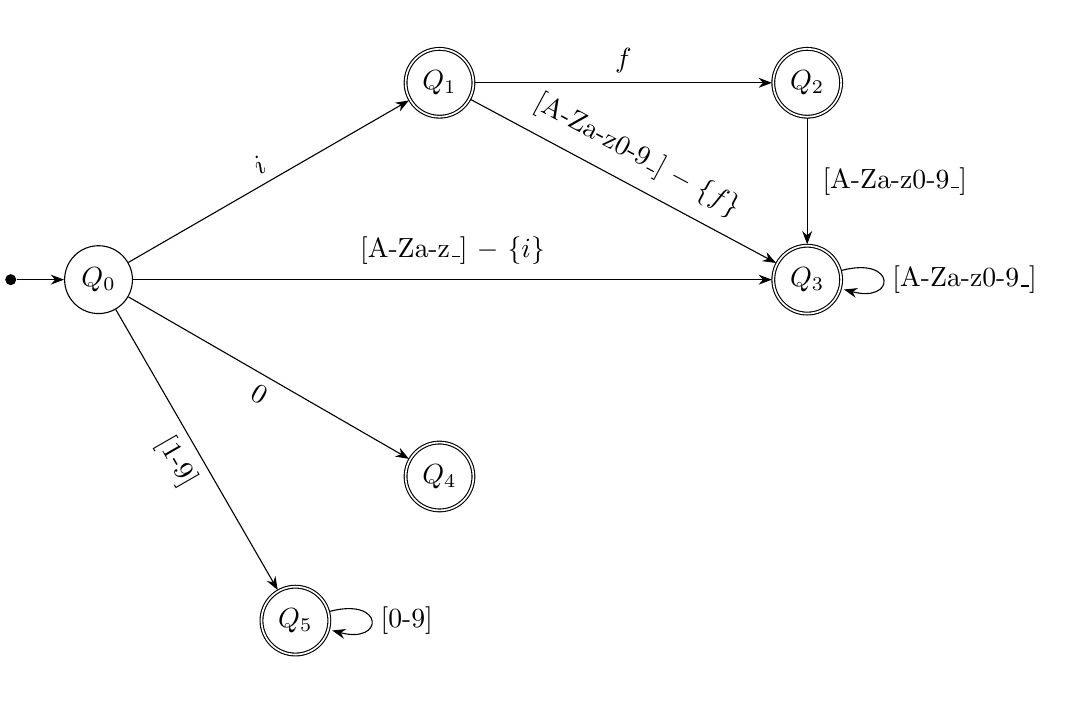
\begin{tikzpicture}[->, >=Stealth, every state/.style={minimum size=8mm}]
\path[use as bounding box] (-0.9,-5) rectangle (12.2,3.2);
\node[state] (Q0) at (0,0) {$Q_0$};
\node[state, accepting] (Q1) at (30:5) {$Q_1$};
\node[state, accepting] (Q2) at (9,2.5) {$Q_2$};
\node[state, accepting] (Q3) at (9,0) {$Q_3$};
\node[state, accepting] (Q4) at (-30:5) {$Q_4$};
\node[state, accepting] (Q5) at (-60:5) {$Q_5$};
\node[circle, fill=black, inner sep=0pt, minimum size=4pt, left=6mm of Q0] (start) {};
\draw (start) -- (Q0);
\path (Q0) edge node[midway, align=center, above, sloped] {$i$} (Q1);
\path (Q0) edge node[midway, align=center, above=2pt] {[A-Za-z\_] $-$ $\{i\}$} (Q3);
\path (Q0) edge node[midway, align=center, below, sloped] {$0$} (Q4);
\path (Q0) edge node[midway, align=center, below, sloped] {[1-9]} (Q5);
\path (Q1) edge node[midway, align=center, above] {$f$} (Q2);
\path (Q1) edge node[midway, align=center, above=2pt, sloped] {[A-Za-z0-9\_] $-$ $\{f\}$} (Q3);
\path (Q3) edge[loop right] node[midway, align=center, right] {[A-Za-z0-9\_]} (Q3);
\path (Q5) edge[loop right] node[midway, align=center, right] {[0-9]} (Q5);
\path (Q2) edge node[midway, align=center, right=2pt] {[A-Za-z0-9\_]} (Q3);
\end{tikzpicture}
}
\end{minipage}
\par\medskip


\subsection{DFA}
\begin{center}
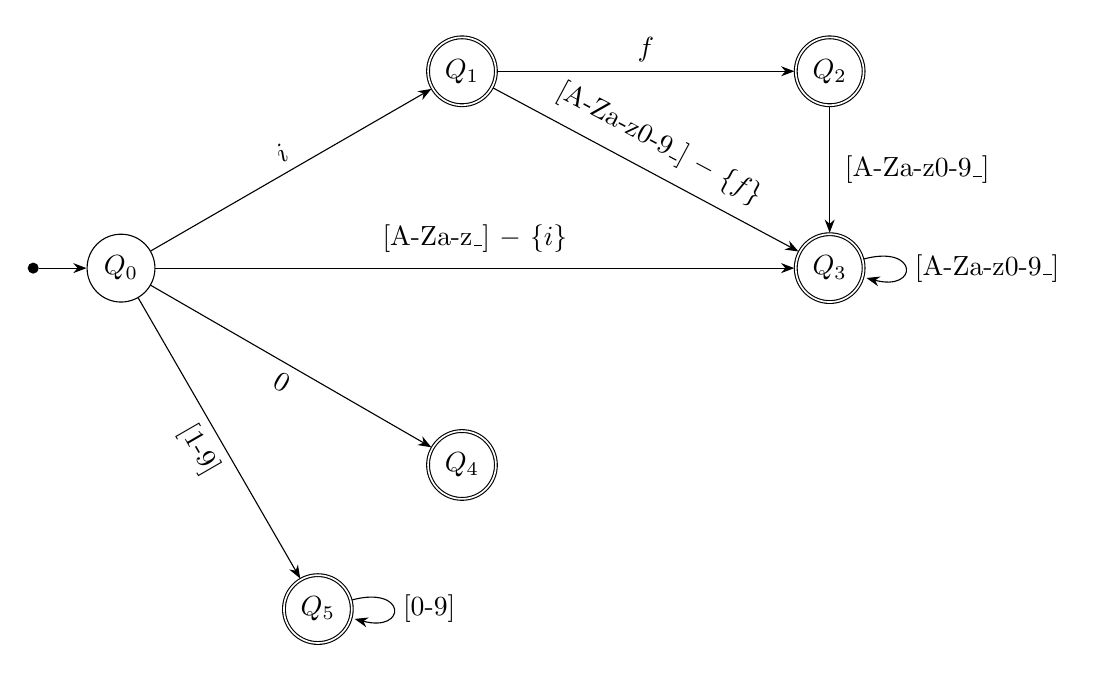
\begin{tikzpicture}[->, >=Stealth, every state/.style={minimum size=8mm}]
\node[state] (Q0) at (0,0) {$Q_0$};
\node[state, accepting] (Q1) at (30:5) {$Q_1$};
\node[state, accepting] (Q2) at (9,2.5) {$Q_2$};
\node[state, accepting] (Q3) at (9,0) {$Q_3$};
\node[state, accepting] (Q4) at (-30:5) {$Q_4$};
\node[state, accepting] (Q5) at (-60:5) {$Q_5$};
\node[circle, fill=black, inner sep=0pt, minimum size=4pt, left=6mm of Q0] (start) {};
\draw (start) -- (Q0);
\path (Q0) edge node[midway, align=center, above, sloped] {$i$} (Q1);
\path (Q0) edge node[midway, align=center, above=2pt] {[A-Za-z\_] $-$ $\{i\}$} (Q3);
\path (Q0) edge node[midway, align=center, below, sloped] {$0$} (Q4);
\path (Q0) edge node[midway, align=center, below, sloped] {[1-9]} (Q5);
\path (Q1) edge node[midway, align=center, above] {$f$} (Q2);
\path (Q1) edge node[midway, align=center, above=2pt, sloped] {[A-Za-z0-9\_] $-$ $\{f\}$} (Q3);
\path (Q3) edge[loop right] node[midway, align=center, right] {[A-Za-z0-9\_]} (Q3);
\path (Q5) edge[loop right] node[midway, align=center, right] {[0-9]} (Q5);
\path (Q2) edge node[midway, align=center, right=2pt] {[A-Za-z0-9\_]} (Q3);
\end{tikzpicture}
\end{center}

\appendix
\section{Appendix: Subset Construction Algorithm}
\begin{center}
\begin{tabular}{r|l}
\textbf{line} & \textbf{operation} \\
\hline
1 & \(\mathtt{D0}:=\varepsilon\mbox{-closure}(\{\mathtt{N0}\})\) \\
2 & \(\mathtt{D}:=\{\mathtt{D0}\}\) \\
3 & \(\mathtt{W}:=\{\mathtt{D0}\}\) \quad\texttt{// worklist} \\
4 & \textbf{while} \(\mathtt{W}\ne\emptyset\): \\
5 & \quad\textbf{remove} \(\mathtt{Q}\) \textbf{from} \(\mathtt{W}\) \\
6 & \quad\textbf{for} \(\alpha\in\Sigma\): \\
7 & \qquad\(\mathtt{T}:=\emptyset\) \\
8 & \qquad\textbf{for} \(\mathtt{S}\in\mathtt{Q}\): \\
9 & \qquad\quad\(\mathtt{T}:=\mathtt{T}\cup\delta_N(\mathtt{S},\alpha)\) \\
10 & \qquad\(\mathtt{T}' := \varepsilon\mbox{-closure}(\mathtt{T})\) \\
11 & \qquad\(\mathtt{D}' := \mathtt{D}\cup\{\mathtt{T}'\}\) \\
12 & \qquad\(\delta_D(\mathtt{Q},\alpha)=\mathtt{T}'\) \quad\texttt{// update} \(\delta_D\) \\
13 & \qquad\textbf{if} \(\mathtt{T}'\notin\mathtt{D}\): \\
14 & \qquad\quad\(\mathtt{W}:=\mathtt{W}\cup\{\mathtt{T}'\}\) \\
15 & \qquad\(\mathtt{D}:=\mathtt{D}'\) \\
16 & \(\mathtt{F\_D}:=\{\mathtt{Q}\in\mathtt{D}\mid\mathtt{Q}\cap\mathtt{F\_N}\ne\emptyset\}\) \quad\texttt{// define} \(\mathtt{F\_D}\) \\
\end{tabular}
\end{center}

\end{document}
